\section{Network Architectures}
\label{sec:networkArchitectures}

One of the first \ac{CNN} architectures was the \textbf{Le-Net5} \cite{LeNet5}.
This \ac{CNN} was proposed to classify handwritten digits.
It used five convolution and pooling layers.
14 years later \ac{CNN}s were rediscovered with the introduction of \textbf{AlexNet} \cite{AlexNet2012} in 2012.
In the \ac{ILSVRC} \cite{ILSVRC15} in 2012, \textbf{AlexNet} outperformed traditional algorithms and showed the potential of \ac{CNN}s.
Consequently, it is often considered as the start of the \ac{CNN} era in the literature.
Since then, research has shown a rapid development of \ac{CNN} architectures, consistently striving for greater accuracy or speed~\cite{networkArchitectureSurvey}.

\vspace{1cm} % Größerer Abstand zwischen den Reihen

\noindent Several major advancements up to now include:

\begin{itemize}
    \item In 2014, two popular architectures were introduced, which are still often used for state-of-the-art comparisons. Firstly, the \textbf{\ac{VGGNet}} \cite{VGGNet2015} used small three-by-three filters and many layers, providing a deep network architecture. Secondly, the \textbf{Inception} network or \textbf{GoogLeNet} \cite{InceptionNet}. To extract features in a range of various scales, this architecture utilized different filter sizes.
    \item In 2015 the \textbf{ResNet} architecture \cite{ResNet} introduced the concept of residual learning with shortcut connections. By skipping layers, this framework enabled the training of deeper networks with over a hundred layers \cite{networkArchitectureSurvey}.
    \item In 2016 \textbf{DenseNets} \cite{DenseNets} was introduced to further deal with the problem of vanishing gradients. This architecture implemented a connection between each layer and every following layer, ensuring maximum information flow \cite{networkArchitectureSurvey}.
    \item In 2017 \textbf{MobileNets} \cite{MobileNetV1, MobileNetV2, MobileNetV3} was developed for applications in mobile devices. Since hardware with limited capabilities is used, the main focus of MobileNet architectures lies on efficiency. Using depth-wise separable convolutions allowed small model sizes and low latencies \cite{networkArchitectureSurvey}.
    \item In 2019 \textbf{EfficientNets} \cite{EfficientNet} was introduced to further explore more significant trade-offs between accuracy and efficiency by using scaling methods for model architectures \cite{networkArchitectureSurvey}. 
\end{itemize}

\vspace{0.5cm} % Größerer Abstand zwischen den Reihen

\noindent Since \ac{CNN}s are part of a rapidly developing research field, more recent architectures are more interesting for this work.
Because they have already solved issues that exist in older models.
Therefore, only the last four mentioned \ac{CNN}s are described in more detail in the following sections.

\subsection{ResNets}

A widely used model architecture in the community is ResNet \cite{ResNet}.
Before this architecture, \ac{CNN}s faced challenges with the vanishing gradient problem, especially in models with a significant depth.
A neural network is generally classified as deep when it includes numerous sequential layers \cite{ResNet}.
ResNet introduced the residual block that is also visualized in \autoref{fig:resnetResidualBlock} to solve that issue.
This block enabled effective training of models with up to 152 layers. Compared to VGGNet, ResNet is 8 times deeper but still less complex.
ResNet showed a significant performance gain and was therefore granted first place in the classification task of the \ac{ILSVRC} 2015.
ResNet is supported in Pytorch, which includes variants with 18, 34, 50, 101, and 152 layers \cite{pytorchresnet}.
However, ResNet models are still resource-intensive because of their size \cite{networkArchitectureSurvey}. 

\begin{figure}[H]
    \centering
    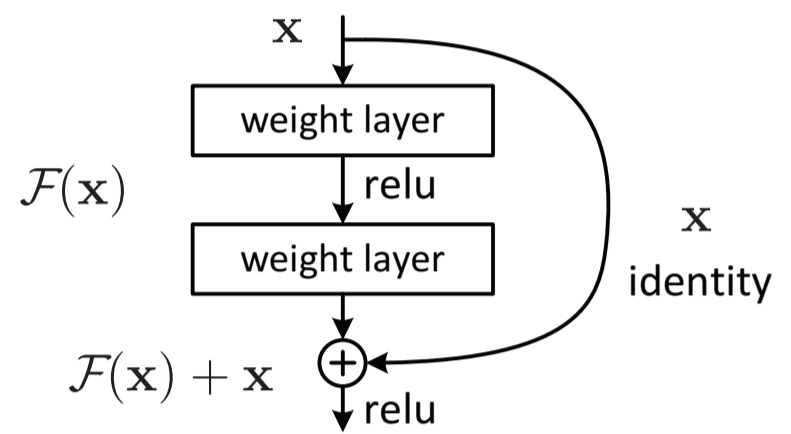
\includegraphics[width=0.5\linewidth]{PICs/backbones/resnet_residualBlock.jpg}
    \caption{ResNet residual block \cite{ResNet}}
    \label{fig:resnetResidualBlock}
\end{figure}

\noindent \autoref{fig:resnetResidualBlock} schematically represents the ResNet's skip connection.
The block has two processes.
One consists of two layers, and the other one performs identity mapping.
After that, the outputs are added together.

\subsection{DenseNets}

DenseNet \cite{DenseNets} further explores skip connections and implemented architecture blocks in which each layer is connected to every following layer.
An example of a so-called "dense block" is shown in \autoref{fig:densenetDenseBlock}.
Compared to ResNet, this model connects outputs via concatenation instead of addition.
Between dense blocks, there are the so-called "transition layers" consisting of one convolutional and then one pooling layer.
This architecture allows deeper \ac{CNN}s, which result in more accuracy and efficiency.
DenseNet showed great results with the introduced technique because their blocks further tackle the vanishing gradient problem with feature reuse.
PyTorch includes DenseNet model variants with 121, 161, 169, 201 \cite{pytorchdensenet}.

\begin{figure}[H]
    \centering
    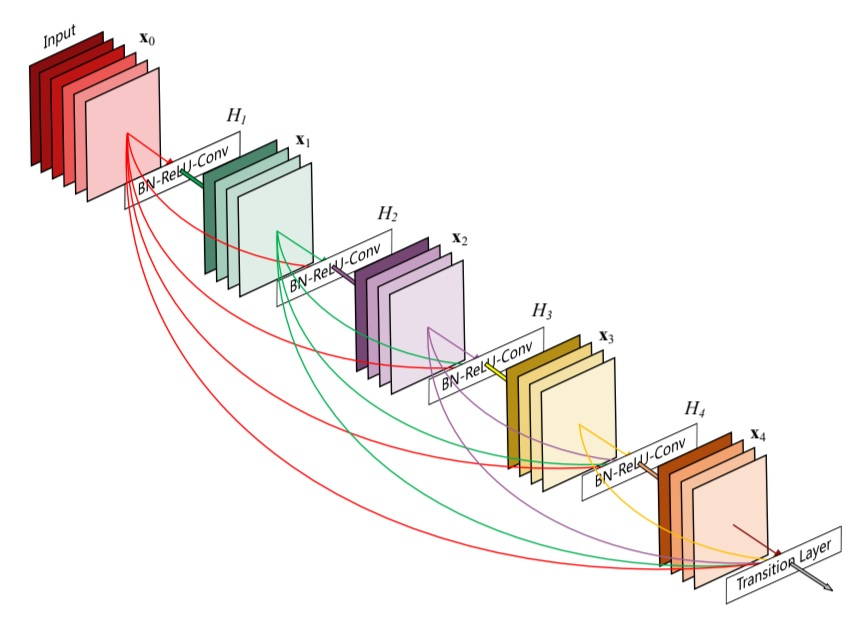
\includegraphics[width=0.6\linewidth]{PICs/backbones/densenet_denseBlock.jpg}
    \caption{DenseNet dense block \cite{DenseNets}}
    \label{fig:densenetDenseBlock}
\end{figure}

\vspace{0.5cm}

\subsection{MobileNets}

The goal of the MobileNet series \cite{MobileNetV3} is to efficiently operate on limited hardware, for example, on mobile devices.
Therefore, the main focus of these models is to be as lightweight as possible \cite{networkArchitectureSurvey}, meaning the reduction of parameters and ensuring real-time capabilities while maintaining comparable accuracy.
There are three versions of MobileNets, each building upon and extending its predecessor.
To achieve a reduced size, version 1 utilizes depth-wise separable convolutions.
These blocks of convolutions consist of two steps. First, a depth-wise convolution, where a kernel is deployed on each channel, followed by a point-wise convolution, where a 1x1 kernel combines the output from the first step \cite{networkArchitectureSurvey}.
MobileNet V2 added a layer with a 1x1 kernel before the depth-wise convolution and a residual connection to create its so-called bottleneck blocks.
A bottleneck block from MobileNetV2 is shown in \autoref{fig:mobileNetV2Block}.

% Bild von MobileNet
\begin{figure}[H]
    \centering
    \begin{subfigure}{0.6\textwidth}
        \centering
        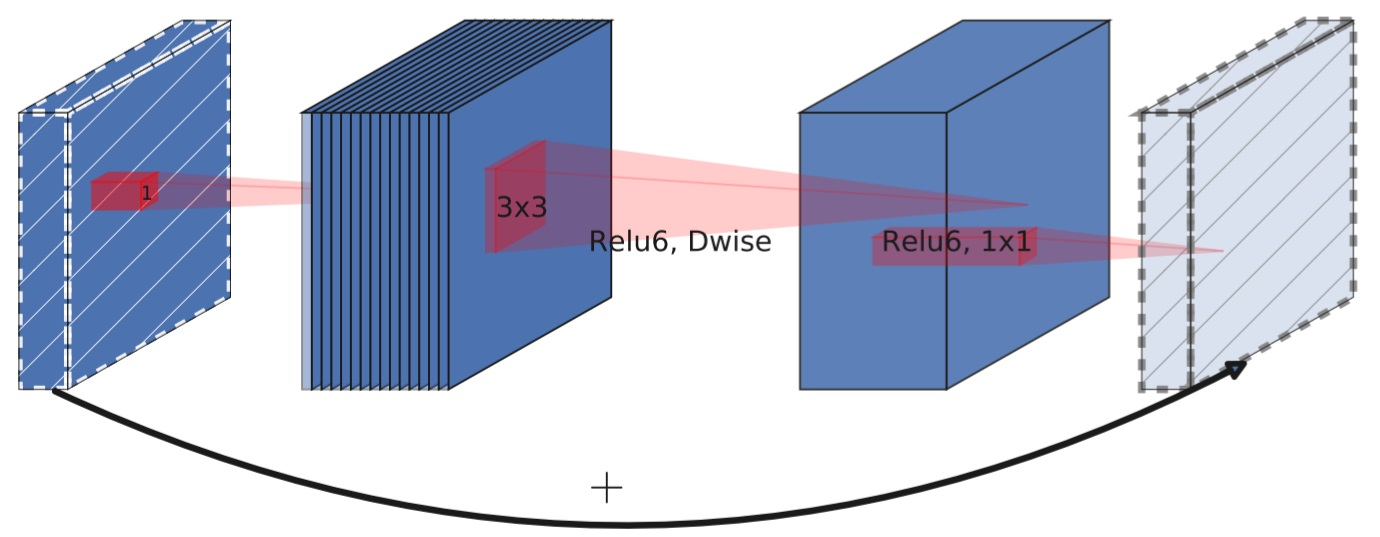
\includegraphics[width=\linewidth, keepaspectratio]{PICs/backbones/mobilenetv2_bottleneck.jpg}
        \caption{}
        \label{fig:mobileNetV2Block}
    \end{subfigure}
    \qquad
    %\hspace*{0.02\textwidth} % Abstand manuell steuern
    \begin{subfigure}{0.6\textwidth}
        \centering
        \vspace{0.8cm}
        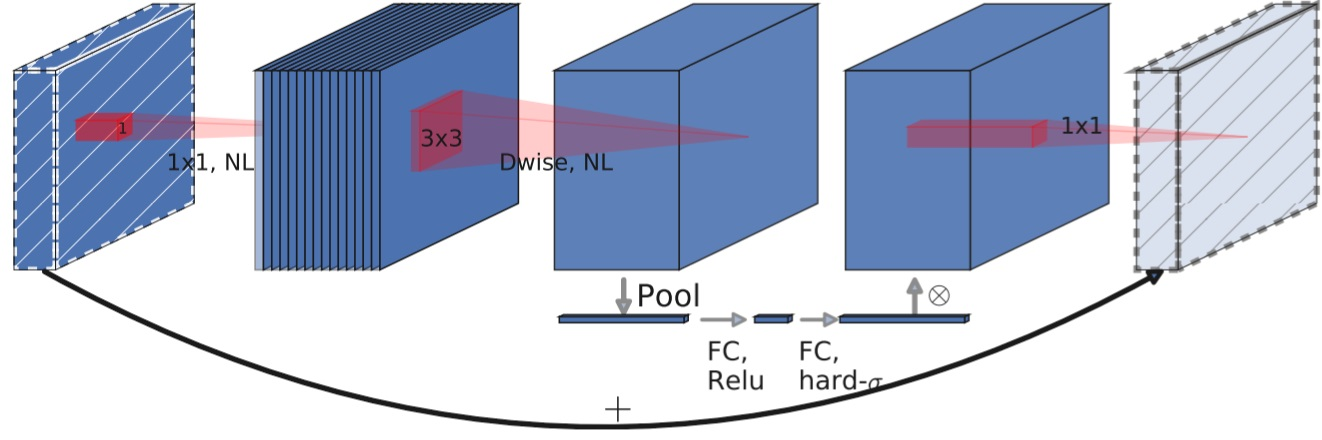
\includegraphics[width=\linewidth, keepaspectratio]{PICs/backbones/mobilenetv3_bottleneck_SE.jpg}
        \caption{}
        \label{fig:mobileNetV3Block}
    \end{subfigure}
    \caption{MobileNet V2 and V3 Blocks \cite{MobileNetV3}: \textbf{(a)} MobileNetV2 bottleneck block, \textbf{(b)} MobileNetV3 bottleneck block with added Squeeze-and-Excite block}
    \label{fig:mobileNetBlocks}
\end{figure}


\noindent MobileNet V3 added optional blocks called Squeeze-and-Excite, which is illustrated in \autoref{fig:mobileNetV3Block}. 
These blocks can be added to any \ac{CNN} and consist of a global pooling layer and two fully connected layers with a ReLu and a Sigmoid activation function, respectively.
After that, the output of this additional block is multiplied by the input feature map of the SE block.
This enables the weighing of specific channels \cite{SqueezeAndExcitation2019}.
Additionally, for the MobileNet V3, a Network Search is used to find optimal network structures and experiments with various activation functions have been conducted \cite{MobileNetV3}.

MobileNets allow flexible usage with the so-called width or in V3 depth multiplier, which is a hyperparameter for controlling the number of feature maps in layers.
MobileNet V1 and V2 additionally offer the resolution multiplier, which controls the resolution of layers.
Both the MobileNetV3\_small and MobileNetV3\_large are supported in PyTorch \cite{pytorchmobilenetv3}.
\clearpage
\subsection{EfficientNets}

EfficientNet \cite{EfficientNet} further investigates methods to find \ac{CNN} architectures optimized for efficiency.
Inspired by MobileNet V3, the models also deploy residual bottleneck convolutions.
\cite{EfficientNet} calls such a block an "MBConv".
Since \cite{EfficientNet} observed the correlation between performance improvement and model scaling, the idea is to strategically adjust a network's depth, width, and resolution.
\autoref{fig:efficientNet_scaled} visualizes these parameters in an example network.
\autoref{fig:efficientNet_networks} shows a network, before (\autoref{fig:efficientNet_baseline}) and after (\autoref{fig:efficientNet_scaled}) scaling is applied.
Consequently, a scaling method is introduced, which uses a so-called "compound coefficient".
The resolution, depth, and width are uniformly scaled with this technique, resulting in eight variants of EfficientNet.
The different versions, starting with B0 and ending with B7, have increasing parameters.
Since this work focuses on lightweight architectures, the first four (B0, B1, B2, B3) are the most interesting models.
All variants of the EfficientNet are included in the PyTorch library \cite{pytorchefficientNets}.


% Bild von EfficientNet
\begin{figure}[H]
    \centering
    \begin{subfigure}{0.4\textwidth}
        \centering
        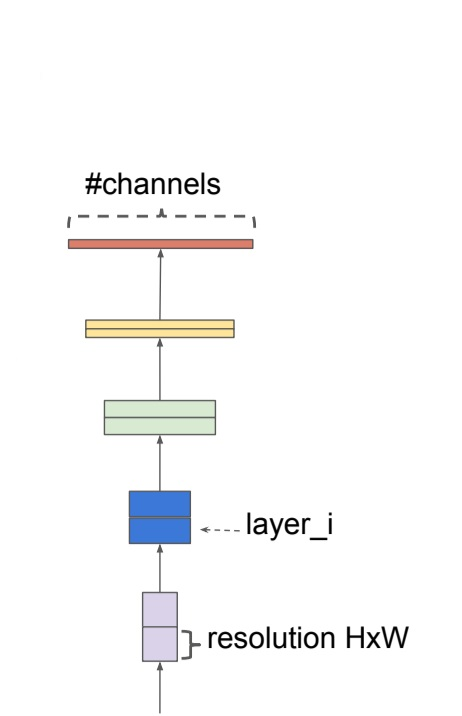
\includegraphics[width=\linewidth, height=7cm, keepaspectratio]{PICs/backbones/EfficientNet_baseline.jpg}
        \caption{Network before scaling method}
        \label{fig:efficientNet_baseline}
    \end{subfigure}
    \qquad
    %\hspace*{0.02\textwidth} % Abstand manuell steuern
    \begin{subfigure}{0.4\textwidth}
        \centering
        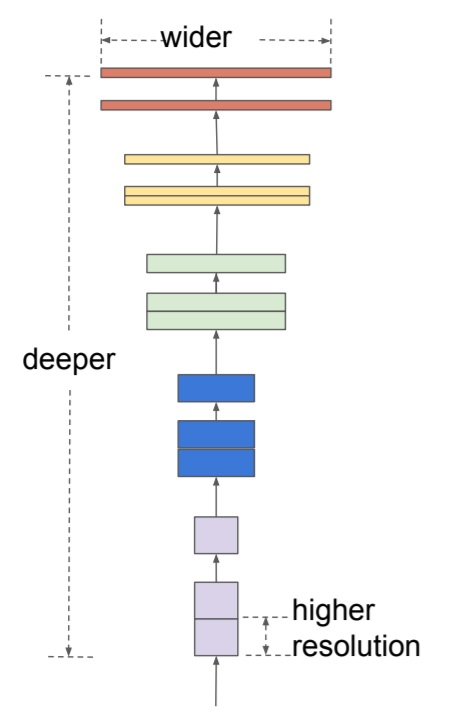
\includegraphics[width=\linewidth, height=7cm, keepaspectratio]{PICs/backbones/EfficientNet_scaling.jpg}
        \caption{Scaling parameters of a network according to \cite{EfficientNet}}
        \label{fig:efficientNet_scaled}
    \end{subfigure}
    \caption{Systematic visualization of scaling parameters of a network \cite{EfficientNet}}
    \label{fig:efficientNet_networks}
\end{figure}